\documentclass[12pt, letterpaper]{article}
\title{Lab Report A2}
\usepackage{graphicx}
\usepackage{amsmath}
\usepackage[margin=1in]{geometry}% Sets 1in margins. 
\usepackage{fancyhdr}			% Creates headers and footers
\usepackage{enumerate}          %These two package give custom labels to
\usepackage[shortlabels]{enumitem}
\author{Aditya Gupta}
\date{\today}
\begin{document}
\maketitle
\newpage
\tableofcontents
\newpage
\section{Introduction}
This lab report explores the data procured by measuring the distance travelled by a rolling ball on an incline surface at regular time intervals.
\section{Raw Data}
The following table contains the data for the collected experiment
\begin{table}[h!]
\centering
\begin{tabular}{|c|c|c|c|}
\hline
\textbf{Trial} & \textbf{Time (s)} & \textbf{Measurement (cm)} \\
\hline
\#1 & 1 & 7.3 \\
    & 2 & 15.7 \\
    & 3 & 32.8 \\
    & 4 & 57.5 \\
    & 5 & 85.6 \\
    & 6 & 113.9 \\
\hline
\#2 & 1 & 8.9 \\
    & 2 & 19.7 \\
    & 3 & 36.5 \\
    & 4 & 61.5 \\
    & 5 & 90.9 \\
    & 6 & 124.4 \\
\hline
\#3 & 1 & 7.9 \\
    & 2 & 18 \\
    & 3 & 34.2 \\
    & 4 & 55.5 \\
    & 5 & 85.4 \\
    & 6 & 128 \\
\hline
\#4 & 1 & 7.6 \\
    & 2 & 20.7 \\
    & 3 & 38.3 \\
    & 4 & 59.8 \\
    & 5 & 87.8 \\
    & 6 & 119.9 \\
\hline
\end{tabular}
\caption{Time and Measurement Data for Trials}
\label{table:measurement_data}
\end{table}

\section{Processed Data}
The first step to processing the data is to obtain the mean of all observations. Here is a sample calculation:
\[
\Sigma_{i=0}^n (d) =\frac{7.3+8.9+7.9+7.6}{4} = 7.9
\]
Calculating all averages,
\begin{table}[h!]
\centering
\begin{tabular}{|c|c|c|c|c|c|}
\hline
\textbf{Time (s)} & \textbf{Trial 1 (cm)} & \textbf{Trial 2 (cm)} & \textbf{Trial 3 (cm)} & \textbf{Trial 4 (cm)} & \textbf{Average (cm)} \\ \hline
1                 & 7.3                   & 8.9                   & 7.9                   & 7.6                   & 7.92                \\ \hline
2                 & 15.7                  & 19.7                  & 18                    & 20.7                  & 18.5                \\ \hline
3                 & 32.8                  & 36.5                  & 34.2                  & 38.3                  & 35.5                \\ \hline
4                 & 57.5                  & 61.5                  & 55.5                  & 59.8                  & 58.6                \\ \hline
5                 & 85.6                  & 90.9                  & 85.4                  & 87.8                  & 87.4                \\ \hline
6                 & 113.9                 & 124.4                 & 128                   & 119.9                 & 121.6                \\ \hline
\end{tabular}
\caption{Measurement Data with Averages for Each Time Point}
\label{table:measurement_data_averages}
\end{table}


Now, to calculate Uncertainty in data, we must calculate the standard deviation of the data. Here is a sample calculation for interval 1:

1. Calculate the mean:
   \[
   \text{Mean} = \frac{7.3 + 8.9 + 7.9 + 7.6}{4} = 7.925
   \]

2. Calculate each deviation from the mean, square it, and then take the average of these squared deviations to find the variance:
   \[
   (7.3 - 7.925)^2 = 0.390625
   \]
   \[
   (8.9 - 7.925)^2 = 0.950625
   \]
   \[
   (7.9 - 7.925)^2 = 0.000625
   \]
   \[
   (7.6 - 7.925)^2 = 0.105625
   \]
   \[
   \text{Variance} = \frac{0.390625 + 0.950625 + 0.000625 + 0.105625}{4} = 0.361875
   \]

3. The standard deviation (SD) is the square root of the variance:
   \[
   \text{SD} = \sqrt{0.361875} \approx 0.6
   \]

Thus, the standard deviation for time interval 1 is approximately \( 0.6016 \, \text{cm} \).


\begin{table}[h!]
\centering
\begin{tabular}{|@{}c@{}|@{}c@{}|@{}c@{}|@{}c@{}|@{}c@{}|@{}c@{}|@{}c@{}|@{}}
\hline
\textbf{Time (s)} & \textbf{Trial 1 (cm)} & \textbf{Trial 2 (cm)} & \textbf{Trial 3 (cm)} & \textbf{Trial 4 (cm)} & \textbf{Average (cm)} & \textbf{SD (cm)} \\ \hline
1                 & 7.3                   & 8.9                   & 7.9                   & 7.6                   & 7.925                 & 0.6016           \\ \hline
2                 & 15.7                  & 19.7                  & 18                    & 20.7                  & 18.525                & 2.2           \\ \hline
3                 & 32.8                  & 36.5                  & 34.2                  & 38.3                  & 35.45                 & 2.2           \\ \hline
4                 & 57.5                  & 61.5                  & 55.5                  & 59.8                  & 58.575                & 2.40           \\ \hline
5                 & 85.6                  & 90.9                  & 85.4                  & 87.8                  & 87.425                & 2.2           \\ \hline
6                 & 113.9                 & 124.4                 & 128                   & 119.9                 & 121.55                & 5.7           \\ \hline
\end{tabular}
\caption{Measurement Data with Averages and Standard Deviations for Each Time Point}

\bigbreak


\end{table}

\section{Non-Linearized Graph of Position vs Time}
    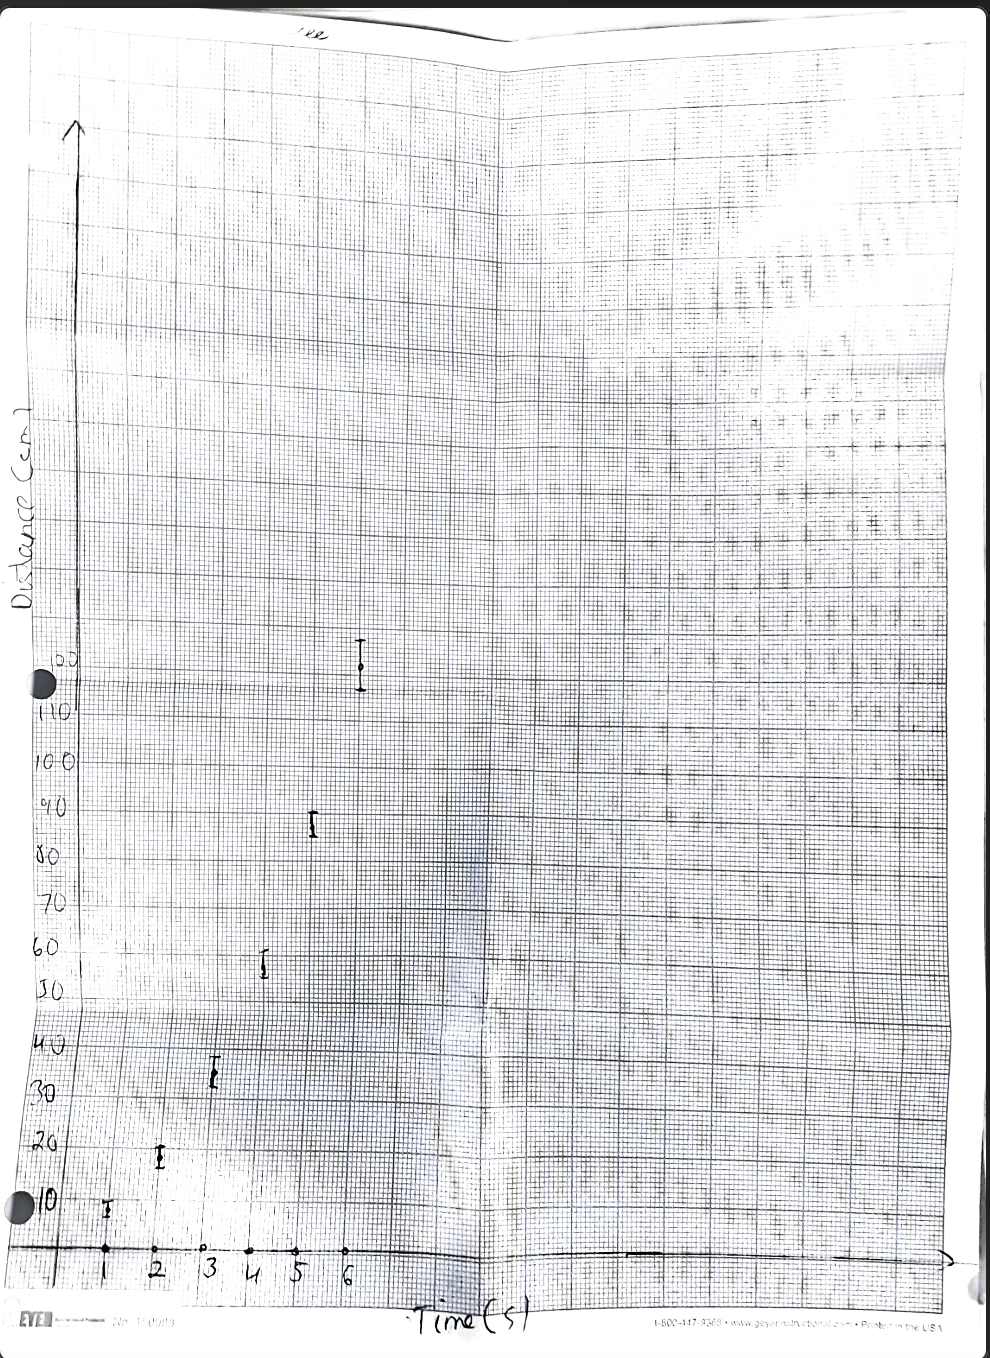
\includegraphics[width=0.75\linewidth]{Phys 141//Lab Reports/unlinearised.png}
    
    As seen in the graph, there is a clear quadratic relation between distance covered and time. 

\section{Linearized Graph of Position vs Time}
To linearize the graph, we plot Distance covered against Time squared. Thus, below is the linearized graph.

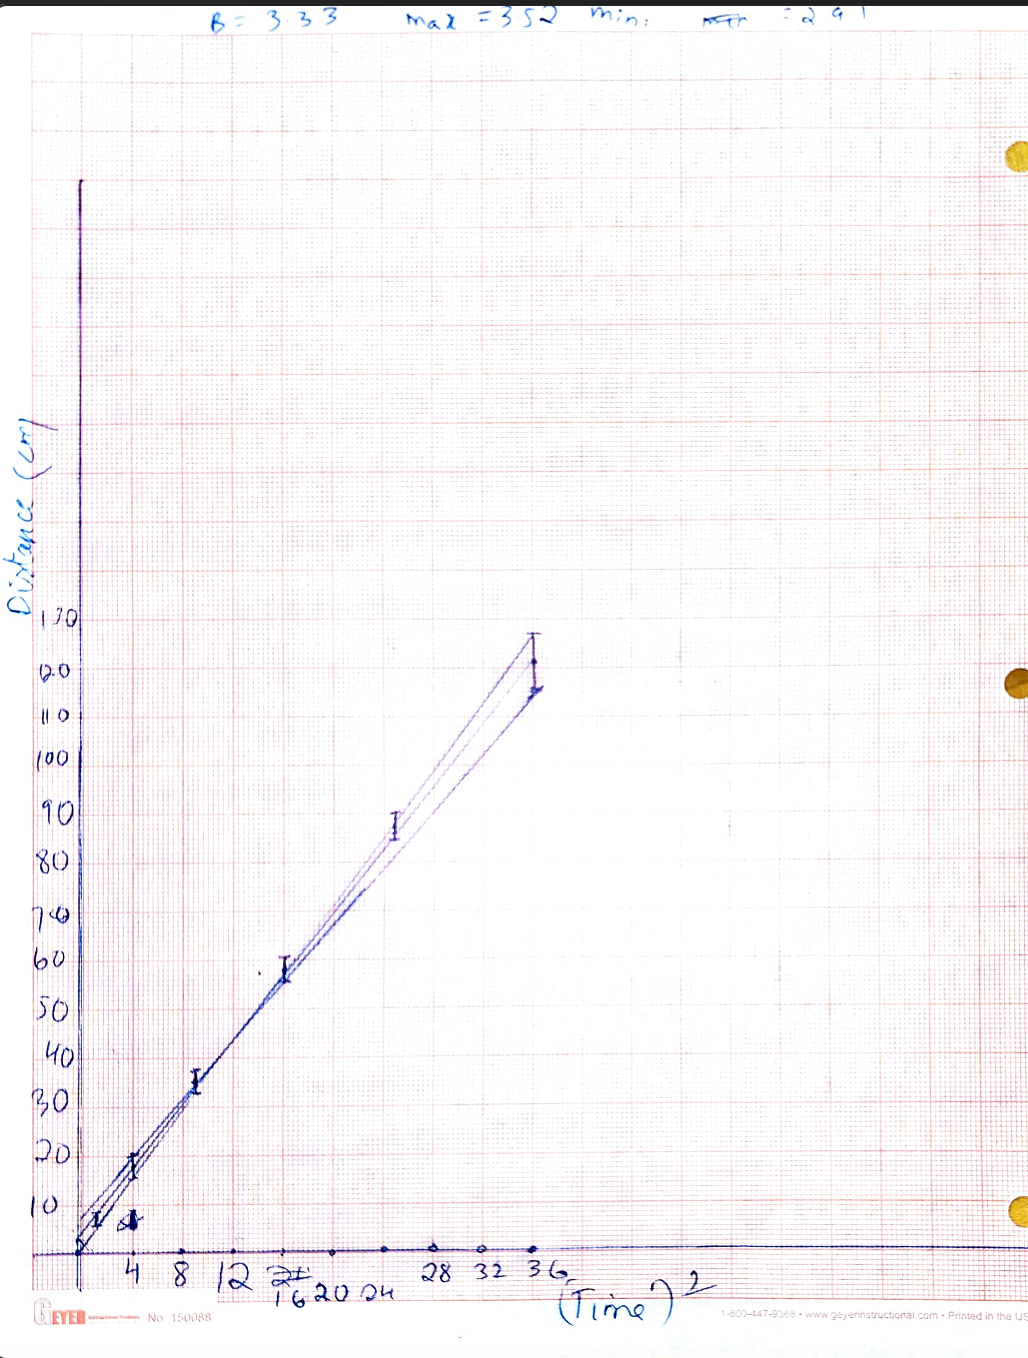
\includegraphics[width=0.75\linewidth]{Phys 141//Lab Reports/linearized.png}

\section{Calculation of Slopes of Best Fits}
\subsection{Best Fit}
We find the equation of the best fit line using points $(36, 121)$ and $(0, 3)$, we first calculate the slope $m$:

\[
m = \frac{y_2 - y_1}{x_2 - x_1} = \frac{3 - 121}{0 - 36} = \frac{-118}{-36} = \frac{59}{18} = 3.3
\]


\subsection{Minimum Slope}
To find the line of minimum slope, we use points $(36, 115)$ and $(0, 7)$:

\[
m = \frac{y_2 - y_1}{x_2 - x_1} = \frac{7 - 115}{0 - 36} = \frac{-107}{-36} = \frac{108}{36} = 3
\]




\subsection{Maximum Slope}
To find the equation of line of maximum slope, we take the points $(36, 126)$ and $(0, 0)$.

\[
m_3= \frac{y_2 - y_1}{x_2 - x_1} = \frac{0 - 126}{0 - 36} = \frac{-126}{-36} = 3.5
\]

\section{Slope Uncertainty}
Our slopes are:
\[
m_{min} = 3
\]
\[
m_{best} = 3.3
\]
\[
m_{max} = 3.5
\]

Thus, our uncertainty in slope is:
\[
\frac{3.5-3}{2} = 0.25
\]

Thus, we can say that our slope is: $3.3 \pm 0.25$. This implies that the acceleration of the ball on the incline was $3.3 \pm 0.25 \text{ cm/}s^2 $ 
\end{document}